\chapter{Literature Review}
\label{chap:lit.review}

\section{Introduction}

\subsection{Recurrent Neural Networks}

Recurrent Neural Networks (RNNs) are in forefront of recent development and advances in \textit{deep learning} by making able neural networks to deal with sequences data, which is a major shortcoming in ANN. If the data is based on sequence of events in a video or text, the traditional neural network can't do reasoning for a single event based on its previous one. To tackle this issue RNNs have loops which enables them to persist the information.

\begin{figure}[p]
	\centering
	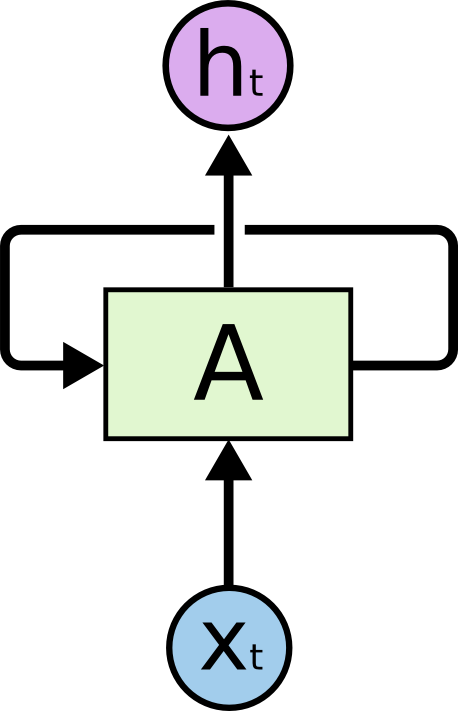
\includegraphics[scale=0.4]{./figs/rnn-rolled}
	\caption[A Rolled Recurrent Neural Networks]{Recurrent Neural Networks (RNNs) uses loops.}
	\label{fig:rnn-rolled}
\end{figure}

As it shown in \textbf{Figure \ref{fig:rnn-rolled}}, a selected neural network, $A$ takes the input $x_t$ and outputs the value of $h_t$. this might not show how data goes from one step to the next one in a same network until you unroll the loop and see chain architecture of recurrent neural networks that makes them the best choice for sequential data, \textbf{Figure \ref{fig:rnn-unrolled}}.

\begin{figure}[p]
	\centering
	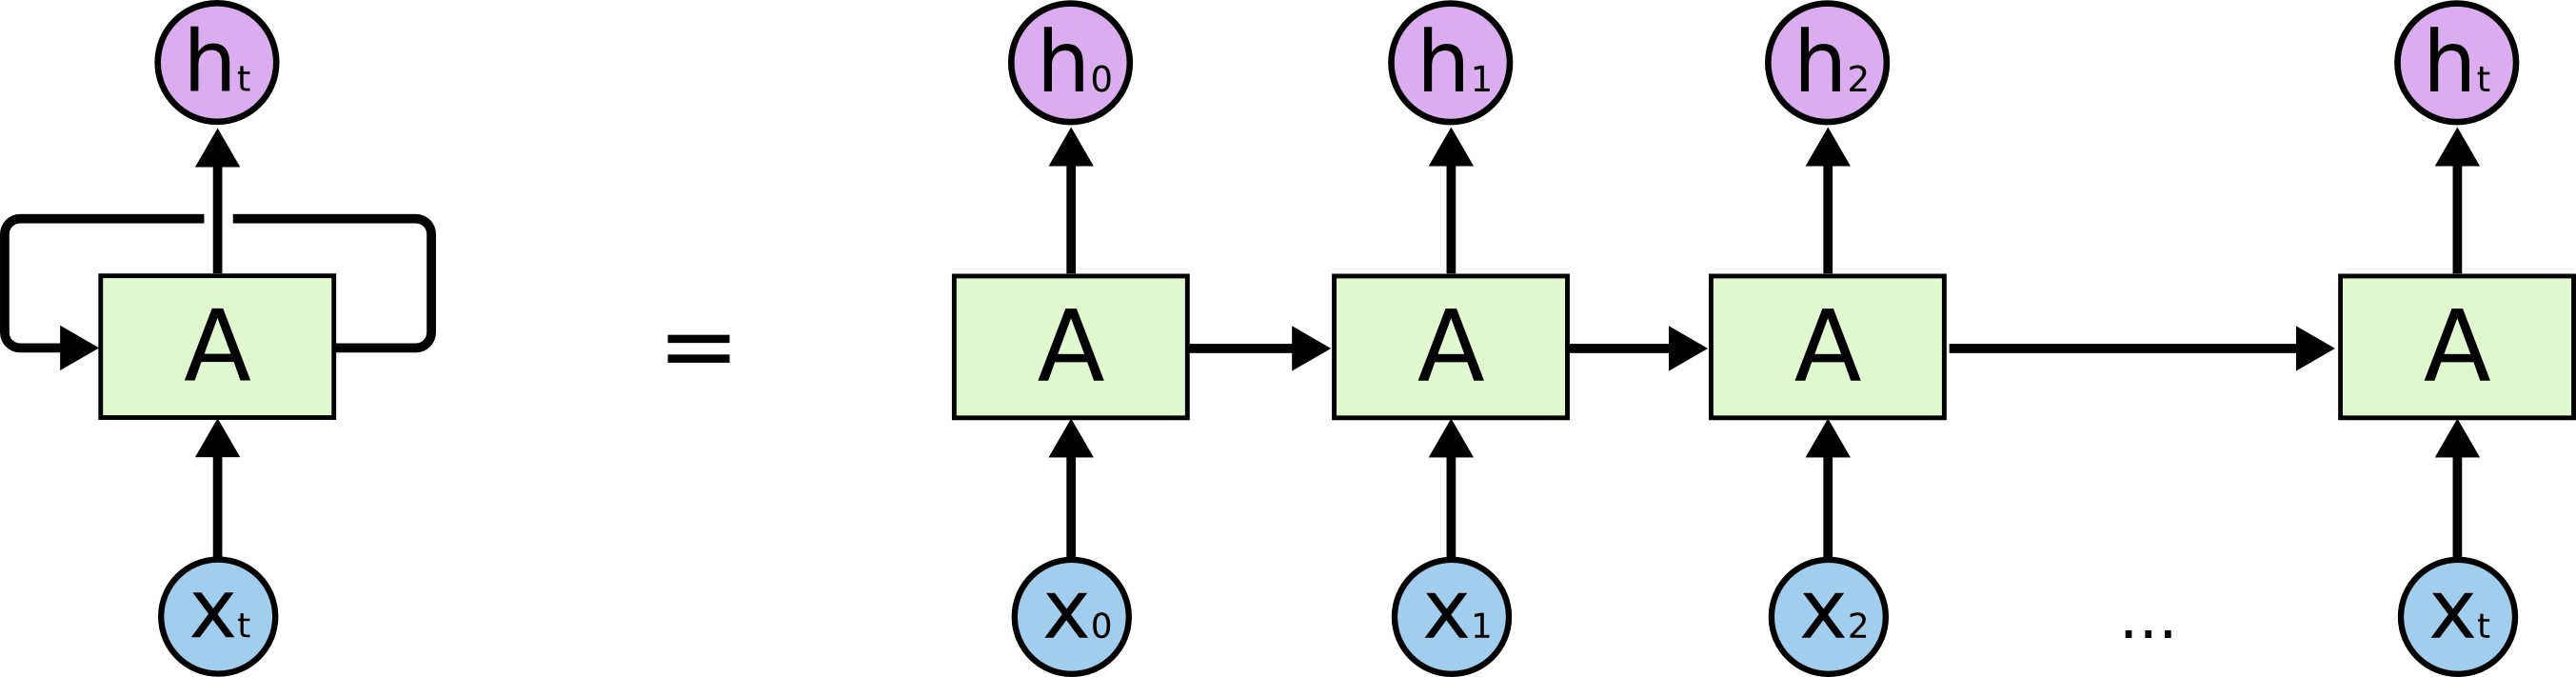
\includegraphics[scale=0.4]{./figs/rnn-unrolled}
	\caption[An Unrolled Recurrent Neural Networks]{An Unrolled Recurrent Neural Networks (RNNs).}
	\label{fig:rnn-unrolled}
\end{figure}

While RNNs is being used in variety of applications from language modeling to image captioning, the essential to all these achievement is the RNN-LSTMs \cite{Hochreiter1997}. An enhanced version of RNNs that outperforms better than the standard RNN.

\subsection{Bayes by Backprop}

Bayes by Backprop \cite{Blundell2015a} is a variational inference scheme for learning the posterior distribution on the weights of a neural network.
The posterior distribution on parameters of the network $\theta \in \mathbb{R}^d$, $q(\theta)$ is typically taken to be a Gaussian with mean parameter $\mu\in \mathbb{R}^d$ and standard deviation parameter $\sigma\in \mathbb{R}^d$, denoted $\mathcal{N}(\theta|\mu,\sigma)$ and it's a diagonal covariance matrix. Where $d$ is the dimensionality of the parameters of the network (usually refers to scale of millions).
Let $\log p(y|\theta, x)$ be the log-likelihood of the neural network, then the network is trained by minimising the variational free energy, where $p(\theta)$ is a prior on the parameters:

\begin{align}
	\label{eq:elbo}
	\mathcal{L}(\theta) &=
	\mathbb{E}_{q(\theta)}\left[\log \frac{q(\theta)}{p(y|\theta, x)p(\theta)}\right],
\end{align}

The \textbf{algorithm \ref{alg:bbb}} shows the Bayes by Backprop Monte Carlo procedure for minimising the above equation with respect to the mean and standard deviation parameters of the posterior $q(\theta)$.

Minimising the variational free energy equation is equivalent to maximising the log-likelihood $\log p(y|\theta, x)$ subject to a KL complexity term in the parameters of the network that acts as a regulariser:

\begin{align}
	\label{eq:klelbo}
	\mathcal{L}(\theta) &=
	- \mathbb{E}_{q(\theta)}\left[\log p(y|\theta, x) \right]
	+ \kl{q(\theta)}{p(\theta)}.
\end{align}

Gaussian process in a case with zero mean prior, the KL term acts as a form of weight decay on the mean parameters, where the rate of weight decay is automatically tuned by the standard deviation parameters of the prior and posterior.

\begin{algorithm}[ht]
	\caption{Bayes by Backprop}
	\label{alg:bbb}
	\begin{algorithmic}
		\STATE{Sample $\epsilon \sim \mathcal{N}(0, I)$, $\epsilon \in \mathbb{R}^d$.}
		\STATE{Set network parameters to $\theta = \mu + \sigma\epsilon$.}
		\STATE{Do forward propagation and backpropagation as normal.}
		\STATE{Let $g$ be the gradient with respect	\label{eq:elbo}
			\mathcal{L}(\theta) &=
			\mathbb{E}_{q(\theta)}\left[\log \frac{q(\theta)}{p(y|\theta, x)p(\theta)}\right], to $\theta$ from backpropagation.} 
		\STATE{Let $g^{KL}_\theta, g^{KL}_\mu, g^{KL}_\sigma$ be the gradients of $\log \mathcal{N}(\theta|\mu, \sigma) - \log p(\theta)$ with respect to $\theta$, $\mu$ and 
			$\sigma$ respectively.} 
		\STATE{Update $\mu$ according to the gradient $g + g^{KL}_\theta + g^{KL}_\mu$.} 
		\STATE{Update $\sigma$ according to the gradient $(g + g^{KL}_\theta) \epsilon + g^{KL}_\sigma$.}
	\end{algorithmic}
\end{algorithm}

The uncertainty afforded by Bayes by Backprop trained networks has been used successfully for training feed-forward NN models for supervised learning and also to help exploration to reinforcement learning agents \cite{Blundell2015a}, \cite{Lipton2016}, \cite{Houthooft2016}, but until now, BBB has not been applied to recurrent neural networks.

\section{Backprop Through Time}
\label{sec:bptt}

As illustrated in \ref{fig:rnn-rolled}, the core of an recurrent neural networks (RNNs), $f$, is a neural network that maps the RNN state at step $t$, $s_t$ and an input observation $x_t$ to a new RNN state $s_{t+1}$, $f: (s_t, x_t) \mapsto s_{t+1}$.

For comparison, an LSTM-powered RNN core \cite{Hochreiter1997} has a state $s_t = (c_t, h_t)$ where $c$ is an internal core state and $h$ is the exposed state. Intermediate gates modulate the effect of the inputs on the outputs, gates like the input gate $i_t$, forget gate $f_t$ and output gate $o_t$. The relationship between the inputs, outputs and internal gates of an LSTM cell can be explained as:

\begin{align*}
i_t &= \sigma(W_i [x_t, h_{t-1}]^T + b_i), \\
f_t &= \sigma(W_f [x_t, h_{t-1}]^T + b_f), \\
c_t &= f_t c_{t-1} + i_t \tanh(W_c [x_t, h_{t-1}] + b_c), \\
o_t &= \sigma(W_o [x_t, h_{t-1}]^T + b_o), \\
h_t &= o_t \tanh(c_t),
\end{align*}

In the above statement, $W_i$ ($b_i$), $W_f$ ($b_f$), $W_c$ ($b_c$) and $W_o$ ($b_o$) are the weights (biases) that are affecting the input gate, forget gate, cell update, and output gate accordingly.

An RNN can be trained on a sequence of $T$ using backpropagation through time where the RNN is unrolled $T$ times like a feed-forward network.
Which can be achieve with forming the feed-forward network with inputs
$x_1, x_2, \dots, x_T$ and initial state $s_0$:

\begin{align}
s_1 &= f(s_0, x_1), \nonumber \\
s_2 &= f(s_1, x_2), \nonumber \\
&\dots \nonumber \\
\label{eq:unroll}
s_T &= f(s_{T-1}, x_T), 
\end{align}

where $s_T$ is the total length (final state) of the RNN.
Referring to the unrolled RNN for $T$ steps as in \eqref{eq:unroll} by $s_{1:T} = F_T(x_{1:T}, s_0)$,
where $x_{1:T}$ is the sequence of input vectors and $s_{1:T}$ is the sequence of corresponding states. However, the truncated version of the algorithm can be seen as taking $s_0$ as the last state of the previous batch, $s_T$.

This RNN parameters are trained in the same way as a feed-forward neural network and a loss is applied to the states $s_{1:T}$ of the RNN, and then backpropagation is being used to update the weights of the trained network.
Since the weights in each of the unrolled step are shared, each weight of the RNN core receives $T$ gradient contributions when the it is unrolled for $T$ steps.


\subsection{Model Confidence}

\subsection{Model Uncertainty and Safety}

\section{State-of-the-Arts}

\section{Limitations}
\begin{enumerate}
\item Mentor~Graphics 2
\begin{enumerate}
\item item 3
\end{enumerate}
\item item 4
\end{enumerate}

\section{Research Gaps}
The processing at layer-5%
